\chapter{Optimization of machine learning models}

This chapter is named optimization due to its contents; here we will account for the choices we compose to optimize the four machine learning algorithms for each of the three approaches outlined in \autoref{sec:data mining}. Initially, that involves finding what information is stored within the databases and the compromise of gathering the information, which further evolves into finding optimal hyperparameters for each approach. Each algorithm has been implemented as seen in \ref{lst:insertAlgorithms}, which is identical to the process of \autoref{chap:validation}.

\begin{comment}
\section{Time of extraction and featurization}

The initial thought behind

\begin{table}[!ht]
\centering
\caption{}
\label{tab:timing-extraction}
\noindent\makebox[\textwidth]{
\begin{tabular}{M{3.0cm} M{4.0cm} M{4.0cm}}
  \hline
  \hline
  Database & Extraction period & Estimated time usage  \\
  \hline
  Materials Project & December $2020$ & $5$ min \\
  Citrine Informatics & December $2020$ & $2$ min  \\
  OQMD & December $2020$ & $3$ min \\
  AFLOW & January $2020$ - February $2021$ & $17$ days \\
  AFLOW-ML & January $2020$ - February $2021$ & $16$ days \\
  JARVIS-DFT & January $2020$ & $5$ min \\
  \hline
  \hline
\end{tabular}
}
\end{table}

\end{comment}
% 139.367, icsd: 52.116, bg: 68141
The first step of this work was to find data from the Materials Project, involving entries that are associated with an ICSD structure and have a PBE-GGA calculated band gap of a minimum of $0.1$eV. Out of $126.335$ existing entries in Materials Project, $48.644$ ($39\%$) were found to have an associated ICSD-structure, while $65.783$ ($52\%$) materials had a calculated band gap of at least $0.1$eV. We found that $25271$ ($20\%$) materials have the band gap minimum and an associated ICSD-structure. It should be noted that these numbers are based on data extraction in December of $2020$, while the extraction from other databases and featurization related to this work was done in the time period of December $2020$ to March $2021$. In February of $2021$, over $30.000$ new materials were added and several materials were deprecated in the V2021.03.22 version of Materials Project\footnote{https://matsci.org/t/materials-project-database-release-log/  (Visited 14.05.2021)}. This update is only included for the insightful approach, which means that the Ferrenti approach and the augmented Ferrenti approach include $77$ ($0.3\%$) more compounds than the insightful approach.

%We note that due to time difference for the data extraction, the test data differs in
%the test data for the insightful approach is done with the overlapping entries of the featurized data set and the V2021.03.22 version of Materials Project. Consequently, the data differs in $77$ ($0.3\%$) compounds from the insightful approach and the two other approaches.

%and therefore the number of entries  in our dataset is based on the latest release in $2020$, which is named V2020.09.08.%, however there are present more than than $2000$ new entries that satisfy the initial MP requirement now.

Two visualizations of two different distributions of the data are found in \autoref{fig:hist_ox} and \autoref{fig:hist_bg}.
The first figure visualizes the distribution of oxide types as a function of the compound type, and reveals that the majority of

\begin{figure}[]
      \centering
      \includegraphics{../predicting-solid-state-qubit-candidates/reports/figures/buildingFeatures/histogram_oxid_nelements.pdf}
      \vspace*{-130mm}
      \caption{Distribution of oxide types as a function of number of elements in compounds in the data. The majority of the entries are found as oxides, while the second most frequent type is not an oxide. }
      \label{fig:hist_ox}
\end{figure}

\begin{figure}[]
      \centering
      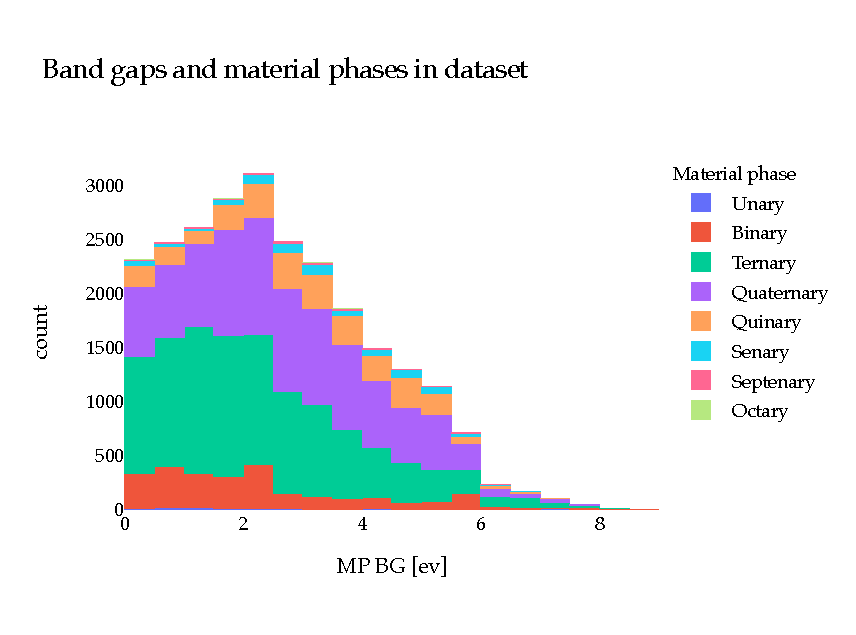
\includegraphics{../predicting-solid-state-qubit-candidates/reports/figures/buildingFeatures/histogram_bg_nelements.pdf}
      \vspace*{-130mm}
      \caption{Distribution of band gaps as function of the compound type in the data. The majority of compounds are ternary and quarternary, while the simpler compounds are few.}
      \label{fig:hist_bg}
\end{figure}

\noindent compounds are either binary, ternary, quarternary, or quinary, hence the majority of the materials are oxides.
This is important to know considering our labeling approaches, in particular the insightful approach where we handpicked suitable entries.
Only a single oxide (ZnO) was deemed a potentially suitable candidate based on observations in Refs. \cite{Zhang2020, Zheng2014, Morfa2012}, which will be interesting to compare towards the different models and approaches.


The second figure (\autoref{fig:hist_bg}) visualize the compound type as a function of band gap, as calculated by Materials Project. Most of the materials present in the data have a band gap lower than $2.3$ eV, where ternary compounds are most prominent. For larger values, we observe that quarternary compounds become dominant for larger band gap values.

\section{Comparing functionals for band gaps}

Since the true size of a band gap is challenging to determine accurately by ab-initio calculations, we provide information regarding five different methods to obtain band gaps as visualized in \autoref{fig:band gaps}. We have extracted experimental band gaps from Citrine Informatics that match the entries made by the initial MP query, involving entries that are associated with an ICSD structure that have a PBE-GGA calculated band gaps of minimum $0.1$ eV.
All the band gaps to the left are found to be common for all databases through screening of correct structure, space group and ICSD-ID, while the figures to the right are only compared to the experimental database of Citrine Informatics.
Notably, it was helpful with the ICSD-tag to find similarities due to databases often have different norms and data structures of descriptors, which proves challenging for comparison of stored calculations.
%If we were to exclude ICSD-tags
If the ICSD-tags had been excluded from the data, it would result in a much larger dataset, however, we found that the determination of similar entries would yield a large deviation when it comes to structures. By including an ICSD-tag, the basis of comparison is reduced but the data exhibits more than $98\%$ identical space group for entries in each database compared to Materials Project.

A very small portion of the data extracted from AFLOW was associated with an ICSD-tag, which yielded only $5$ similar entries to the other databases, and therefore we have excluded the database from further consideration.

In \autoref{fig:band gaps}, we observe each entry marked as black or blue dots. The dotted lines visualize the optimal ratio of the estimated band gap to experimental values, while the red lines show a linear least-square fit to the data with the colored area being the $95\%$ confidence interval. The data that constitute the left figures are based on $82$ similar entries, while the right figures constitute of more entries depending on the respective database. The data restriction was due to a small experimental database.

Initially, we wanted to include the figures to the right in the attempt of reducing the confidence interval with increasing the data points, but instead

\clearpage
\begin{figure}[ht!]
    \centering
    \begin{subfigure}[t]{1\textwidth}
        \centering
        \input{../predicting-solid-state-qubit-candidates/reports/figures/bandgaps/mp.tex}
        \caption{}
    \end{subfigure}%

    \begin{subfigure}[t]{1\textwidth}
        \centering
        \input{../predicting-solid-state-qubit-candidates/reports/figures/bandgaps/oqmd.tex}
        \caption{}
    \end{subfigure}

    \begin{subfigure}[t]{1\textwidth}
        \centering
        \input{../predicting-solid-state-qubit-candidates/reports/figures/bandgaps/aflowml.tex}
        \caption{}
    \end{subfigure}
\end{figure}

\begin{figure}[t!]\ContinuedFloat
    \centering
    \begin{subfigure}[t]{1\textwidth}
        \centering
        \input{../predicting-solid-state-qubit-candidates/reports/figures/bandgaps/jarvis_tbmbj.tex}
        \caption{}
    \end{subfigure}%

    \begin{subfigure}[t]{1\textwidth}
        \centering
        \input{../predicting-solid-state-qubit-candidates/reports/figures/bandgaps/jarvis_opt.tex}
        \caption{}
    \end{subfigure}
    \vspace*{-130mm}
    \caption{Comparison of reported experimental band gaps to those calculated by (a) Materials Project, (b) Open Quantum Materials Database, (c) AFLOW-ML, (d) JARVIS-DFT (TB-mBJ) and (e) JARVIS-DFT (OptB88). The figures to the left show reported band gaps that have been found to be common through all databases, while the figures to the right are only common with experimentally reported values from Citrine Informatics. All entries have been extracted in the period of January to March of $2021$. }
    \label{fig:band gaps}
\end{figure}

\clearpage

\noindent we find that the uncertainty of the confidence interval increase for all HT- methods.
This is due to the fact that the majority of the new entries are found for low band gap values, where the mismatch between experimental and calculated values is the largest.
The discrepancy seems to be the largest for values under $5$ eV, where entries are either calculated to have a very large band gap and the experimental values report a very low band gap, or the opposite.
The data extracted from the experimental database is not associated with an ICSD-entry, space group, or structure. Therefore, we cannot accurately determine if the experimental data is based on an identical material as found in the HT-databases. However, the same data of experimental values have been considered through other articles \cite{Ward2018, Ferrenti2020}.

Notably, the functional applied for Materials Project are found to underestimate the band gap with $30-60\%$ while OQMD underestimates the band gap by $25-55\%$. AFLOW-ML also severely underestimates the band gap by $30-60\%$, but additionally has problems to accurately predict if a material is a metal or not. Many materials with both experimental and ab-initio calculations that showed a band gap of more than $1$ eV were predicted as metals by AFLOW-ML. JARVIS-DFT, on the other hand, was found to underestimate the band gap by $20-60\%$ for the OptB88 and $0-30\%$ for TB-mBJ functionals.



%Similar to the results of \citeauthor{Ferrenti2020} \cite{Ferrenti2020}, we find


\section{Technical details on ML classifiers}

%In this section we will provide technical details on the classifiers considering the training process. For each approach, we will apply combinations of principal components ranging from just one to several and look at the resulting implications. For each approach we can end up with over twenty different optimalization processes, which in total could potentially result in over sixty  in total. Therefore, we will not make an extensive analysis for every model, but emphasis important distinctions between the models and provide background for principal choices made. However, it should be noted that an an extensive automated analysis is distributed through the MIT license at the Github repository \textit{predicting-solid-state-qubit-candidates} \cite{Ohebbi2021}.

In the evaluation of the approaches, we apply a $5\times 5$ stratified cross-validation when iterating through the hyperparameter combinations. We acknowledge that the three approaches exhibit imbalanced datasets, similar to the dataset in the validation chapter. Adjusting the class balance for the latter case helped with reducing the variance in a very small data set and the class ratio of $1:9$. In this section, we find all three approaches to have substantially larger datasets than the cubic perovskite dataset, thus we choose to not apply any technique for balancing the classes. Instead, we apply four different algorithms to compare them to each other, and use four different evaluation metrics to estimate how the classifiers are performing. %Interestingly,   %There is a wide field of other techniques that deal with the vulnerabilites of imbalanced datasets \cite{Lemaitre2016}, but they a
% Thus, we choose to not apply any technique for balancing the classes, but rather find the compromise

For random forest, gradient boost, and decision tree, we found that by adjusting most of the available parameters responded to severe overfitting. Therefore, most parameters are the default values defined by Scikit-learn. The only parameter that we found that could potentially improve the evaluation metric $F1$ was the maximum number of depth for the trees grown, which we adjusted between $1$ and $8$. For logistic regression, we choose to adjust the regularization strength with seven logarithmical adjusted values $10^{-3}$ to $10^{5}$, and use either $200$ or $400$ iterations to reach convergence.

When searching for the optimal number of principal components, we iterated over every odd number of principal components from $1$ to the upper restricted number which defines an accumulated variance of $95\%$ from the principal component analysis. Due to a large number of principal components, we end up fitting $25$ folds for each of $1232$ parameter combinations, totaling up to $30800$ individual models, just for logistic regression for one approach. This serves as an additional motivator to keep the models simple, and accordingly shows how easy an initial complex step might evolve into an unfeasible amount of information. Therefore, we will not make an extensive analysis for every model, but emphasize important distinctions between the general models and provide background for principal choices made. However, it should be noted that a larger automated analysis is distributed through the MIT license at the Github repository \textit{predicting-solid-state-material-hosts} \cite{Ohebbi2021}.


\subsection{The Ferrenti approach}

We visualize the grid search for the optimal number of principal components in \autoref{fig:01-pca}, where we present the mean accuracy on the training set, and the balanced accuracy, precision, recall, and F1-score on the test set as a function of principal components used in the models. For each principal component, we visualize the optimal combination of hyperparameters based on the F1-score in the model. Common to all models is the improvement of scores up to around $50$ principal components, where random forest and the decision tree slowly start to overfit for larger values. For decision trees, we observe a large fluctuation for principal components larger than $100$. The F1-score is not varying as much as the other metrics due to an increasing number of positive predictions. This means that the accuracy of positive predictions is dominating the overall accuracy measurement, and we would expect a large amount of training data to be predicted as positive candidates for those combinations. However, we see that the fluctuations are smaller in size for the optimal number of principal components.

The random forest model is similar to the decision tree model, which also shows signs of overfitting for larger values of principal components. The recall score is unaltered for increasing principal components, but consequently, we find the precision declining due to a large amount of predicted false positives.  However, as a result of an ensemble of decision trees, it shows smaller signs of overfitting than the indications seen by the decision tree algorithm.

Gradient boost, on the other hand, experiences minor changes for a larger number of principal components, where the optimal number of components marked could be $50$ principal components less without any remarks to the model's metrics. Notably, only a few principal components yield almost $100\%$ training accuracy for GB, while not showing any clear sign of overfitting. Similarly, logistic regression shows signs of almost a perfect classifier with high scores for all metrics.

\clearpage

\begin{figure}[ht!]
  \begin{subfigure}[b]{1.0\textwidth}
    \centering
    \input{../predicting-solid-state-qubit-candidates/reports/figures/pca-scores/03-insightful-approach-176-label.tex}
  \end{subfigure}
  \par\bigskip
  \begin{subfigure}[b]{0.5\textwidth}
    \input{../predicting-solid-state-qubit-candidates/reports/figures/pca-scores/01-ferrenti-approach-176-LOG.tex}
    \caption{}
    \label{fig:q1-LOG}
  \end{subfigure}%
  \hfill
  \begin{subfigure}[b]{0.5\textwidth}
    \input{../predicting-solid-state-qubit-candidates/reports/figures/pca-scores/01-ferrenti-approach-176-DT.tex}
    \caption{}
    \label{fig:q1-DT}
  \end{subfigure}

  \begin{subfigure}[b]{0.5\textwidth}
    \input{../predicting-solid-state-qubit-candidates/reports/figures/pca-scores/01-ferrenti-approach-176-RF.tex}
    \caption{}
    \label{fig:q1-RF}
  \end{subfigure}%
  \hfill
  \begin{subfigure}[b]{0.5\textwidth}
    \input{../predicting-solid-state-qubit-candidates/reports/figures/pca-scores/01-ferrenti-approach-176-GB.tex}
    \caption{}
    \label{fig:q1-GB}
  \end{subfigure}
  \vspace*{-130mm}
  \caption{{Four figures displaying hyperparameter search for the Ferrenti approach. The best estimator is visualized for all hyperparameters as a function of principal components during a grid search with a $5\times5$ stratified cross-validation, and the dotted lines mark the optimal hyperparameter-combination. Train stands for normal training accuracy, while test is the balanced accuracy on the test set. Precision, recall, and F1 scores are based on the test set. The number of principal components that explain the $95\%$ accumulated variance is $144$, while the optimal model is found using the F1-score.}}
  \label{fig:01-pca}
\end{figure}

\clearpage

\begin{table}[!ht]
\centering
\caption{A table of the optimal number of principal components and the respective scores (standard deviation) for the Ferrenti approach, as visualized in the dash-dotted line in \autoref{fig:01-pca}.}
\label{tab:01-pc}
\noindent\makebox[\textwidth]{
\begin{tabular}{M{1.0cm} M{1.0cm} M{2.0cm} M{2.0cm}M{2.0cm}M{2.0cm} }
  \hline
  \hline
   Model & PC & Mean test &  Mean precision & Mean recall & mean F1\\
  \hline
  LOG & $171$ & $0.98(0.012)$ & $0.98(0.011)$ & $0.99(0.007)$ & $0.99(0.007)$ \\
  DT & $37$   & $0.77(0.034)$ & $0.84(0.034)$ & $0.85(0.044)$ & $0.84(0.022)$ \\
  RF & $53$   & $0.87(0.027)$ & $0.88(0.022)$ & $0.98(0.010)$ & $0.93(0.014)$ \\
  GB & $107$  & $0.92(0.016)$ & $0.92(0.015)$ & $0.98(0.010)$ & $0.95(0.009)$ \\
  \hline
\end{tabular}
}
\end{table}



\begin{wrapfigure}{R}{0.5\textwidth}

  \begin{subfigure}[b]{1.0\textwidth}
  \input{../predicting-solid-state-qubit-candidates/reports/figures/pca-scores/03-insightful-approach-176-label.tex}
  \end{subfigure}

  \begin{subfigure}[b]{1.0\textwidth}
  \input{../predicting-solid-state-qubit-candidates/reports/figures/grid-scores/01-ferrenti-approach-GB.tex}
  \end{subfigure}
  \vspace*{-130mm}
  \caption{Parameter search for the Ferrenti approach regarding maximum depth for gradient boost for several metrics, where the error bars visualize the standard deviation.}
  \label{fig:gb-01-overfit}
\end{wrapfigure}

\noindent In \autoref{tab:01-pc}, we find the precise measurements for each evaluation metric for the optimal number of principal components, which is visualized as dotted lines in \autoref{fig:01-pca}. The relevant hyperparameters for logistic regression were the maximum iterations, which was set at $400$, and the regulariation term, which was found optimal at $0.46$. For random forest and decision trees, we find the maximum depth of $7$, while gradient boost was found to overfit for deeper depths, as visualized in \autoref{fig:gb-01-overfit} and thus we found an optimal compromise at $4$. We find that the best performing model is logistic regression, but is dependent on a large amount of principal components. Random forest and gradient boost perform comparably, with and F1-score of $0.93$ and $0.95$, respectively. However, it seems that only logistic regression is able to improve for additional principal components after the first $100$.



%The specific scores for the arbitrary number of principal components is found in the Appendix \autoref{appendix:Optimalization}.  The lower plots visualizes the explained variance ratio, both accumulated and stepwise.


In \autoref{fig:01-fi}, we visualize how the models interpret the principal components that are sorted in descending order by the explained variance, found through a $5\times 5$ stratified cross-validation. To reach the $95\%$ accumulated explained variance, a total of $144$ principal components needs to be involved. We have visualized the first $25$ since this captures the most important information, and we note that most of the important features are within the first five principal components.

For logistic regression, we have visualized the mean fitted coefficients and the standard variation in \autoref{fig:01-fi}. Large positive or negative coefficients can be considered increasingly important, where positive (negative) coefficients will contribute making positive (negative) predictions. In the three next

\begin{wrapfigure}{r}{0.5\textwidth}
  \begin{subfigure}[b]{0.5\textwidth}
    \centering
    \input{../predicting-solid-state-qubit-candidates/reports/figures/feature-importance/01-ferrenti-approachLOG-final.tex}
    \label{fig:01-fi-a}
  \end{subfigure}%

  \begin{subfigure}[b]{0.5\textwidth}
    \centering
    \input{../predicting-solid-state-qubit-candidates/reports/figures/feature-importance/01-ferrenti-approachDT-final.tex}
    \label{fig:01-fi-b}
  \end{subfigure}%

  \begin{subfigure}[b]{0.5\textwidth}
    \centering
    \input{../predicting-solid-state-qubit-candidates/reports/figures/feature-importance/01-ferrenti-approachRF-final.tex}
    \label{fig:01-fi-c}
  \end{subfigure}%

  \begin{subfigure}[b]{0.5\textwidth}
    \centering
    \input{../predicting-solid-state-qubit-candidates/reports/figures/feature-importance/01-ferrenti-approachGB-final.tex}
    \label{fig:01-fi-d}
  \end{subfigure}%

  \begin{subfigure}[b]{0.5\textwidth}
    \centering
    \input{../predicting-solid-state-qubit-candidates/reports/figures/feature-importance/01-ferrenti-approachPC-final.tex}
    \label{fig:01-fi-e}
  \end{subfigure}%

  \vspace*{-130mm}
  \caption{Five figures visualizing different parameters for the $25$ most principal components ranked in descending order by the explained variance for the Ferrenti approach. The panels show the logistic regression coefficients, decision tree feature importance, random forest feature importance, gradient boost feature importance, and explained variance that is retained by choosing each of the eigenvectors. }
  \label{fig:01-fi}
\end{wrapfigure}

\noindent figures, namely the decision tree, random forest, and gradient boost, we visualize the mean impurity-based feature importance, along with the standard deviation. Importantly, we observe that the single most important feature for all models is the fifth principal component. Interestingly, by selecting the highest values in this eigenvector, we find that the corresponding features originate from the DFT band gap of elemental solid among elements in the composition as calculated by OQMD.

After the first ten principal components, we observe that the models adapt the other principal components with varying degrees. Logistic regressions coefficients experience large fluctuations, but the three remaining models find the first and second principal components important. In order of importance, we observe that the second component's largest values correspond to the electronegativity, ionic property, and covalence radius among the elements in the composition. The aggregations are either calculated as minimum, mean, standard deviation, or maximum. While the first principal component has by far the largest explained variance, it does not provide any specific information of which features it represents. Some of the features represent the period in the periodic table, structural packing efficiency, and atomic weights of the components. However, we are unable to confirm the prominent features due to small variations.

%a variety of features are represented, such as the rows that a composition in the periodic table represents, structural packing efficiency and atomic weights of the components, but we are unable to confirm the prominent features due to small variations.

We note that looking at feature importance can be regarded as misleading for data involving correlated features, but we consider the analysis safe due to the projection of the original data to orthogonal vectors, known as principal components, which results in uncorrelated features.



\subsection{The augmented Ferrenti approach}

For the augmented Ferrenti approach, we find the parameter grid search for principal components visualized in \autoref{fig:02-pca}. All models experience an almost perfect recall score for the $1$ principal component due to the largely imbalanced dataset with $2141$ suitable and $684$ unsuitable candidates, which is a ratio of $75:25 \%$. This result comes as a consequence of the models being able to correctly label many suitable candidates compared to the number of unsuitable candidates. On the other hand, we find a small precision for the $1$ component since the model predicts many materials, both actually labeled suitable and unsuitable, as suitable candidates, and the latter case is particularly large. This trend is revealed when looking at the balanced accuracy score. For all figures, it remains the lowest score of the evaluation metrics largely due to the inaccuracy of true negatives for the cross-validations. Therefore, one can argue that we should use the balanced accuracy score for evaluation and not the F1 score, but the choice is independent of the evaluation metric since the optimal F1 score is also the optimal balanced accuracy score for all figures.


\begin{table}[!ht]
\centering
\caption{A table of the optimal number of principal components and the respective scores (standard deviation), as visualized in the dash-dotted line in \autoref{fig:02-pca}.}
\label{tab:02-pc}
\noindent\makebox[\textwidth]{
\begin{tabular}{M{1.0cm} M{1.0cm} M{2.0cm} M{2.0cm}M{2.0cm}M{2.0cm} }
  \hline
  \hline
   Model & PC & Mean test &  Mean precision & Mean recall & mean F1\\
  \hline
  LOG & $175$ & $0.98(0.008)$ & $0.99(0.004)$ & $0.99(0.004)$ & $0.99(0.003)$ \\
  DT & $25$   & $0.69(0.034)$ & $0.86(0.015)$ & $0.93(0.021)$ & $0.90(0.008)$ \\
  RF & $25$   & $0.70(0.028)$ & $0.86(0.011)$ & $1.00(0.003)$ & $0.93(0.006)$ \\
  GB & $93$   & $0.85(0.025)$ & $0.93(0.011)$ & $0.99(0.004)$ & $0.96(0.007)$ \\
  \hline
\end{tabular}
}
\end{table}

\noindent Overall, the search for optimal hyperparameters in \autoref{fig:02-pca} for the augmented Ferrenti approach bears resemblance to \autoref{fig:01-pca} for the Ferrenti approach. Logistic regression performs optimally for many principal components, and is the only model that continues to improve with an increasing number of components. The decision tree model exhibit a large fluctuation of scores, where the number of false positives is dominating the balanced accuracy score. Random forest exhibit fewer fluctuations compared to the decision tree as a consequence of the ensemble decision trees, while gradient boost does not improve after around $100$ principal components.

\begin{wrapfigure}{R}{0.5\textwidth}

  \begin{subfigure}[b]{1.0\textwidth}
  \input{../predicting-solid-state-qubit-candidates/reports/figures/pca-scores/03-insightful-approach-176-label.tex}
  \end{subfigure}

  \begin{subfigure}[b]{1.0\textwidth}
  \input{../predicting-solid-state-qubit-candidates/reports/figures/grid-scores/02-augmented-ferrenti-approach-LOG.tex}
  \end{subfigure}
  \vspace*{-130mm}
  \caption{Parameter search for the augmented Ferrenti approach regarding regularization parameter for logistic regression for several metrics, where the error bars visualize the standard deviation.}
  \label{fig:log-02-overfit}
\end{wrapfigure}

The optimal hyperparameters are summarized in \autoref{tab:02-pc}. We find that the logistic regression model with $175$ principal components perform more or less like a perfect classifier with overall high scores. The decision tree and random forest models have similar balanced accuracy scores with $0.69$ and $0.70$, respectively, due to challenges associated with predicting true negative labels for $25$ principal components. Lastly, we find that gradient boost performs optimally at $93$ principal components with a balanced accuracy score of $0.85$.

\begin{figure}[ht!]
  \begin{subfigure}[b]{1.0\textwidth}
    \centering
    \input{../predicting-solid-state-qubit-candidates/reports/figures/pca-scores/03-insightful-approach-176-label.tex}
  \end{subfigure}
\par\bigskip
  \begin{subfigure}[b]{0.5\textwidth}
    \input{../predicting-solid-state-qubit-candidates/reports/figures/pca-scores/02-augmented-ferrenti-approach-176-LOG.tex}
    \caption{}
    \label{fig:q2-LOG}
  \end{subfigure}%
  \hfill
  \begin{subfigure}[b]{0.5\textwidth}
    \input{../predicting-solid-state-qubit-candidates/reports/figures/pca-scores/02-augmented-ferrenti-approach-176-DT.tex}
    \caption{}
    \label{fig:q2-DT}
  \end{subfigure}

  \begin{subfigure}[b]{0.5\textwidth}
    \input{../predicting-solid-state-qubit-candidates/reports/figures/pca-scores/02-augmented-ferrenti-approach-176-RF.tex}
    \caption{}
    \label{fig:q2-RF}
  \end{subfigure}%
  \hfill
  \begin{subfigure}[b]{0.5\textwidth}
    \input{../predicting-solid-state-qubit-candidates/reports/figures/pca-scores/02-augmented-ferrenti-approach-176-GB.tex}
    \caption{}
    \label{fig:q2-GB}
  \end{subfigure}
  \vspace*{-130mm}
  \caption{{Four figures displaying hyperparameter search for the augmented Ferrenti approach. The best estimator is visualized for all hyperparameters as a function of principal components during a grid search with a $5\times5$ stratified cross-validation, and the dotted lines mark the optimal hyperparameter-combination. Train stands for normal training accuracy, while test is the balanced accuracy on the test set. Precision, recall, and F1 scores are based on the test set. The number of principal components that explain the $95\%$ accumulated variance is $159$, while the optimal model is found using the F1-score.}}
  \label{fig:02-pca}
\end{figure}

The relevant hyperparameters of logistic regression were the regularization strength, which was set to $0.46$, as visualized in \autoref{fig:log-02-overfit}, and we set maximum iterations at $400$. Smaller regularization values resulted in worse scores, while increasing values did not notably alter the results. The decision tree and random forest found an optimal maximum depth of $7$, where smaller values resulted in low precision but high recall. Therefore, the choice was made to facilitate a compromise between precision and recall. For gradient boost, we find the optimal maximum depth as $4$ due to a decline in overall metrics for increasing depth except for training accuracy, which could potentially result in overfitting.

%Four figures displaying hyperparameter search for the second approach. The best estimator is visualized for all hyperparameters as a function of principal components during a grid search with a 5x5 stratified cross-validation. The lower plots visualizes the explained variance ratio, both accumulated and stepwise. The dotted lines marks the optimal hyperparameter-combination, while the error bars display the standard deviation.

The interpretation of feature importance for the Ferrenti approach is substantially more difficult than in the Ferrenti approach. We find for logistic regression and decision trees that no feature is different than any other in the cross-validation due to a large variety of accuracy. However, we find that random forest and gradient boost experience the fifth principal component as important. Similar to the Ferrenti approach, the corresponding features with the highest value for the first principal component originates the DFT band gap of elemental sold among elements in the composition.

\subsection{The insightful approach}

Lastly, we turn to the insightful approach, which involves $404$ unsuitable and $187$ suitable candidates in the imbalanced training set. However, in contrast to the two other datasets, the majority of the entries are labeled as unsuitable candidates.

The grid search for the optimal number of principal components is visualized in \autoref{fig:03-pca}. Interestingly, we find that all models experience high scores for just a few principal components, where $1$ principal component earns at least $0.93$ scores for all evaluation metrics. This information was also revealed for an earlier two-dimensional visualization of a scatter plot showing the two most important principal components in \autoref{fig:2dscatterplotpca}, and consequently can make the models find the optimal decision boundary more easily.

Logistic regression experiences improvement of all scores for an increasing number of principal components, yet only up $5\%$ in scores compared to the one-dimensional representation of one principal component. Thus, one can argue if the increase in performance is worth it considering a one-dimensional representation with just a few percentage losses of performance. However, with multiple principal components, we find the largest increase in precision, which is a sign that the one-dimensional representation tends to wrongly predict candidates as suitable when they are in fact unsuitable. The decision tree and the random forest models exhibit the best performance for just a few principal components, and experience considerably overfitting for larger values. Gradient boost, in contrast to the two other approaches, also experiences the best performance for a few principal components.

\begin{table}[!ht]
\centering
\caption{A table of the optimal number of principal components and the respective scores (standard deviation) for the insightful approach, as visualized in the dash-dotted line in \autoref{fig:03-pca}.}
\label{tab:03-pca}
\noindent\makebox[\textwidth]{
\begin{tabular}{M{1.0cm} M{1.0cm} M{2.0cm} M{2.0cm}M{2.0cm}M{2.0cm} }
  \hline
  \hline
   Model & PC & Mean test & Mean precision & Mean recall  & mean F1\\
  \hline
  LOG & $61$  & $0.99(0.011)$ & $0.97(0.032)$ & $0.99(0.016)$ & $0.98(0.018)$ \\
  DT & $9$    & $0.96(0.019)$ & $0.95(0.040)$ & $0.95(0.033)$ & $0.95(0.026)$ \\
  RF & $27$   & $0.98(0.020)$ & $0.97(0.033)$ & $0.97(0.031)$ & $0.97(0.026)$ \\
  GB & $13$   & $0.97(0.016)$ & $0.96(0.036)$ & $0.97(0.029)$ & $0.96(0.022)$ \\
  \hline
\end{tabular}
}
\end{table}

\noindent The optimal hyperparameters are summarized in \autoref{tab:03-pca}, where all models exhibit high evaluation metrics. Importantly, we find the difference in the number of principal components as most prominent, where logistic regression finds an optimum at $61$ with the F1-score of $0.98$. The decision tree model uses only $9$ principal components to achieve an F1 score of $0.95$, while random forest needs $27$ principal components to gain an F1 score of $0.97$.

\begin{figure}[ht!]
  \begin{subfigure}[b]{1.0\textwidth}
    \centering
    \input{../predicting-solid-state-qubit-candidates/reports/figures/pca-scores/03-insightful-approach-176-label.tex}
  \end{subfigure}
  \par\bigskip
  \begin{subfigure}[b]{0.5\textwidth}
    \input{../predicting-solid-state-qubit-candidates/reports/figures/pca-scores/03-insightful-approach-176-LOG.tex}
    \caption{}
    \label{fig:q3-LOG}
  \end{subfigure}%
  \hfill
  \begin{subfigure}[b]{0.5\textwidth}
    \input{../predicting-solid-state-qubit-candidates/reports/figures/pca-scores/03-insightful-approach-176-DT.tex}
    \caption{}
    \label{fig:q3-DT}
  \end{subfigure}
  \begin{subfigure}[b]{0.5\textwidth}
    \input{../predicting-solid-state-qubit-candidates/reports/figures/pca-scores/03-insightful-approach-176-RF.tex}
    \caption{}
    \label{fig:q3-RF}
  \end{subfigure}%
  \hfill
  \begin{subfigure}[b]{0.5\textwidth}
    \input{../predicting-solid-state-qubit-candidates/reports/figures/pca-scores/03-insightful-approach-176-GB.tex}
    \caption{}
    \label{fig:q3-GB}
  \end{subfigure}

  \vspace*{-130mm}
  \caption{{Four figures displaying hyperparameter search for the insightful approach. The best estimator is visualized for all hyperparameters as a function of principal components during a grid search with a $5\times5$ stratified cross-validation, and the dotted lines mark the optimal hyperparameter-combination. Train stands for normal training accuracy, while test is the balanced accuracy on the test set. Precision, recall, and F1-scores are based on the test set. The number of principal components that explain the $95\%$ accumulated variance is $103$, while the optimal model is found using the F1-score.}}
  \label{fig:03-pca}
\end{figure}

\begin{wrapfigure}{r}{0.5\textwidth}
  \begin{subfigure}[b]{0.5\textwidth}
    \centering
    \input{../predicting-solid-state-qubit-candidates/reports/figures/feature-importance/03-insightful-approachLOG-final-2.tex}
    \label{fig:03-fi-a}
  \end{subfigure}%

  \begin{subfigure}[b]{0.5\textwidth}
    \centering
    \input{../predicting-solid-state-qubit-candidates/reports/figures/feature-importance/03-insightful-approachDT-final-2.tex}
    \label{fig:03-fi-b}
  \end{subfigure}%

  \begin{subfigure}[b]{0.5\textwidth}
    \centering
    \input{../predicting-solid-state-qubit-candidates/reports/figures/feature-importance/03-insightful-approachRF-final-2.tex}
    \label{fig:03-fi-c}
  \end{subfigure}%

  \begin{subfigure}[b]{0.5\textwidth}
    \centering
    \input{../predicting-solid-state-qubit-candidates/reports/figures/feature-importance/03-insightful-approachGB-final-2.tex}
    \label{fig:03-fi-d}
  \end{subfigure}%

  \begin{subfigure}[b]{0.5\textwidth}
    \centering
    \input{../predicting-solid-state-qubit-candidates/reports/figures/feature-importance/03-insightful-approachPC-final-2.tex}
    \label{fig:03-fi-e}
  \end{subfigure}%

  \vspace*{-130mm}
  \caption{Five figures visualizing different parameters for the $15$ most principal components ranked in descending order by the explained variance for the insightful approach. The panels show the logistic regression coefficients, decision tree feature importance, random forest feature importance, gradient boost feature importance, and explained variance that is retained by including each of the eigenvectors. }
  \label{fig:03-fi}
\end{wrapfigure}

\noindent Lastly, gradient boost performs optimally at $13$ principal components with a mean F1-score of $0.96$. The relevant hyperparameters were the regularization term for logistic regression, which was set to $0.021$, and the maximum number of iterations as $400$. The decision tree uses an maximum depth of $6$, where larger values increased the training accuracy but not any other metric. Random forest was set with a maximum depth of $6$, and gradient boost was given $4$.

The insightful approach differs in many aspects from the Ferrenti or augmented Ferrenti approach. Firstly, we find that the number of principal components necessary to obtain $95\%$ variance is reduced to $103$ components, which is $41$ and $56$ less than the Ferrenti or augmented Ferrenti approach, respectively. Thus, the variance of the training set is found to be described with fewer principal components, indicating a simpler model.

Secondly, we find that the first principal component is by far the most important feature for all models, as visualized in \autoref{fig:03-fi}. This is part of the reason why we experience a large accuracy for only a single feature, seen in \autoref{fig:03-pca}. The first principal component's corresponding features are challenging to explain due to small variations of values. However, it differs when it comes to which top features the first principal component describes, which includes bond orientational parameters, coordination numbers, and radial distribution function of a compound's crystal system.

Thirdly, the insightful approach differs in how much explained variation is retained by the first component, which is $21\%$, while it is $14\%$ for the Ferrenti approach and $11\%$ for the augmented Ferrenti approach. We find the difference striking considering the approaches share the same ultimate goal, but where the training set apparently constitutes of large variations.

\begin{figure}[h!]
    \centering
    \includegraphics[trim={2.8cm 0cm 0cm 0cm},clip, scale=1]{../predicting-solid-state-qubit-candidates/reports/figures/pca-3d-plots/GB-3d-iso-train.pdf}
  \vspace*{-140mm}
  \caption{A three-dimensional scatter plot visualizing the labeled training data and the isosurface of gradient boost's decision boundary. Limegreen indicates suitable candidates, while tomato corresponds to unsuitable candidates. The isosurface represents the probability of a prediction.}
  \label{fig:3d-iso}
\end{figure}

\noindent Due to high accuracy for few principal components, we seize the occasion and visualize a scatter plot of the training data in \autoref{fig:3d-iso}. The tomato color visualizes unsuitable candidates, while limegreen corresponds to suitable candidates. Additionally, we have visualized an isosurface representing the decision boundary of an optimized gradient boost for the three most important principal components. Due to a rather sharp transition, we have restricted the probability down to $0.05\%$ of being labeled a suitable candidate, and the remaining area without isosurface is considered unfit for what we are looking for. We can observe that the model easily distinguishes most of the points, but is not able to capture all of the variations in the data.

Importantly, the visualization allows us to shape a picture of the mapping by the principal component analysis. There are mainly three large clusters of data points where the largest is composed of different structures of ZnS, second largest SiC, and the smallest cluster C. % where the largest constitute of all the variations of ZnS and the other of SiC.
Close to the ZnS-cluster, we find ZnSe, ZnTe, CdS, and GaAs, involving both two and three-dimensional strucutures.
%From this, it is clear that the decision tree is not able to distinguish between two and three-dimensional structures.
The SiC-cluster is mostly by itself, with the closest entries being AlN. The cluster consisting of C, however, is more spread out than the two latter and is accompanied by BN. Close to the decision boundary, we find many entries of Si and GaN. On the edge of the border are some of the oxides, such as ZnO, while by crossing the boundary we find oxides such as CoO and SiO$_2$, and the ionic compound NaCl. Interestingly, we find the two-dimensional suitable candidates MoS$_2$, WS$_2$, and WSe$_2$ close together but far into the area of unsuitable candidates.

During the $5\times 5$ cross-validation, we find that all models except for logistic regression are able to predict the true label of unsuitable candidates over $50 \%$ of the time.
The logistic regression model consistently predicts an orthorhombic structured C (mp-$568410$) and hexagonal CoO (mp-$19128$) as suitable candidates, while in fact being labeled as unsuitable. However, all models are able to predict the true labels of all suitable candidates over $50\%$ of the time.

%The logistic regression model predicts the two-dimensional materials MoS$_2$, WS$_2$ and WSe$_2$ as unsuitable candidates consistently. Of the suitable candidates, we find that the decision tree model wrongly predicts the true labels of complex or nano-structures of C, GaAs, SiC, CoO and Si more than $50\%$ of the time. Random forest and gradient boost correctly predicts the true labels of all candidates more than $50\%$ of the time, while logistic regression misses out on the two-dimensional strucutres GaAs and SiC.

%from the trainthree principal components and the
